\documentclass[aspectratio=169,10pt,xcolor=svgnames,compress]{beamer} 
% Explicación de las opciones:
% aspectratio es para que tenga formato 16:9
% 10pt es el tamaño de la fuente por defecto
% xcolor=svgnames selecciona el esquema de colores a utilizar
% compress trata de achicar todas las barras de navegación
% Agregar handout a las opciones, para tener una versión imprimible.

\input{tex/diapo_encabezado.tex}
% tikzlibrary.code.tex
%
% Copyright 2010-2011 by Laura Dietz
% Copyright 2012 by Jaakko Luttinen
%
% This file may be distributed and/or modified
%
% 1. under the LaTeX Project Public License and/or
% 2. under the GNU General Public License.
%
% See the files LICENSE_LPPL and LICENSE_GPL for more details.

% Load other libraries
\usetikzlibrary{shapes}
\usetikzlibrary{fit}
\usetikzlibrary{chains}
\usetikzlibrary{arrows}

% Latent node
\tikzstyle{latent} = [circle,fill=white,draw=black,inner sep=1pt,
minimum size=40pt, font=\fontsize{25}{25}\selectfont, node distance=2]
% Observed node
\tikzstyle{obs} = [latent,fill=gray!25]
% Invisible node
\tikzstyle{invisible} = [latent,minimum size=0pt,color=white, node distance=0]
% Constant node
\tikzstyle{const} = [rectangle, inner sep=0pt, node distance=0.1]
%state
\tikzstyle{estado} = [latent,minimum size=8pt,node distance=0.4]
%action
\tikzstyle{accion} =[latent,circle,minimum size=5pt,fill=black,node distance=0.4]


% Factor node
\tikzstyle{factor} = [rectangle, fill=black,minimum size=10pt, draw=black, inner
sep=0pt, node distance=1]
% Deterministic node
\tikzstyle{det} = [latent, rectangle]

% Plate node
\tikzstyle{plate} = [draw, rectangle, rounded corners, fit=#1]
% Invisible wrapper node
\tikzstyle{wrap} = [inner sep=0pt, fit=#1]
% Gate
\tikzstyle{gate} = [draw, rectangle, dashed, fit=#1]

% Caption node
\tikzstyle{caption} = [font=\footnotesize, node distance=0] %
\tikzstyle{plate caption} = [caption, node distance=0, inner sep=0pt,
below left=5pt and 0pt of #1.south east] %
\tikzstyle{factor caption} = [caption] %
\tikzstyle{every label} += [caption] %

\tikzset{>={triangle 45}}

%\pgfdeclarelayer{b}
%\pgfdeclarelayer{f}
%\pgfsetlayers{b,main,f}

% \factoredge [options] {inputs} {factors} {outputs}
\newcommand{\factoredge}[4][]{ %
  % Connect all nodes #2 to all nodes #4 via all factors #3.
  \foreach \f in {#3} { %
    \foreach \x in {#2} { %
      \path (\x) edge[-,#1] (\f) ; %
      %\draw[-,#1] (\x) edge[-] (\f) ; %
    } ;
    \foreach \y in {#4} { %
      \path (\f) edge[->,#1] (\y) ; %
      %\draw[->,#1] (\f) -- (\y) ; %
    } ;
  } ;
}

% \edge [options] {inputs} {outputs}
\newcommand{\edge}[3][]{ %
  % Connect all nodes #2 to all nodes #3.
  \foreach \x in {#2} { %
    \foreach \y in {#3} { %
      \path (\x) edge [->,#1] (\y) ;%
      %\draw[->,#1] (\x) -- (\y) ;%
    } ;
  } ;
}

% \factor [options] {name} {caption} {inputs} {outputs}
\newcommand{\factor}[5][]{ %
  % Draw the factor node. Use alias to allow empty names.
  \node[factor, label={[name=#2-caption]#3}, name=#2, #1,
  alias=#2-alias] {} ; %
  % Connect all inputs to outputs via this factor
  \factoredge {#4} {#2-alias} {#5} ; %
}

% \plate [options] {name} {fitlist} {caption}
\newcommand{\plate}[4][]{ %
  \node[wrap=#3] (#2-wrap) {}; %
  \node[plate caption=#2-wrap] (#2-caption) {#4}; %
  \node[plate=(#2-wrap)(#2-caption), #1] (#2) {}; %
}

% \gate [options] {name} {fitlist} {inputs}
\newcommand{\gate}[4][]{ %
  \node[gate=#3, name=#2, #1, alias=#2-alias] {}; %
  \foreach \x in {#4} { %
    \draw [-*,thick] (\x) -- (#2-alias); %
  } ;%
}

% \vgate {name} {fitlist-left} {caption-left} {fitlist-right}
% {caption-right} {inputs}
\newcommand{\vgate}[6]{ %
  % Wrap the left and right parts
  \node[wrap=#2] (#1-left) {}; %
  \node[wrap=#4] (#1-right) {}; %
  % Draw the gate
  \node[gate=(#1-left)(#1-right)] (#1) {}; %
  % Add captions
  \node[caption, below left=of #1.north ] (#1-left-caption)
  {#3}; %
  \node[caption, below right=of #1.north ] (#1-right-caption)
  {#5}; %
  % Draw middle separation
  \draw [-, dashed] (#1.north) -- (#1.south); %
  % Draw inputs
  \foreach \x in {#6} { %
    \draw [-*,thick] (\x) -- (#1); %
  } ;%
}

% \hgate {name} {fitlist-top} {caption-top} {fitlist-bottom}
% {caption-bottom} {inputs}
\newcommand{\hgate}[6]{ %
  % Wrap the left and right parts
  \node[wrap=#2] (#1-top) {}; %
  \node[wrap=#4] (#1-bottom) {}; %
  % Draw the gate
  \node[gate=(#1-top)(#1-bottom)] (#1) {}; %
  % Add captions
  \node[caption, above right=of #1.west ] (#1-top-caption)
  {#3}; %
  \node[caption, below right=of #1.west ] (#1-bottom-caption)
  {#5}; %
  % Draw middle separation
  \draw [-, dashed] (#1.west) -- (#1.east); %
  % Draw inputs
  \foreach \x in {#6} { %
    \draw [-*,thick] (\x) -- (#1); %
  } ;%
}



% Las siguientes líneas definen el footline.
\makeatletter
\setbeamertemplate{footline}
{
  \leavevmode%
  \hbox{%
    \begin{beamercolorbox}[wd=.26\paperwidth,ht=2.25ex,dp=1ex,left]{author in head/foot}%
      \hspace*{2em}\usebeamerfont{author in head/foot}\insertauthor
    \end{beamercolorbox}%
    \begin{beamercolorbox}[wd=.48\paperwidth,ht=2.25ex,dp=1ex,center]{title in head/foot}%
      \usebeamerfont{title in head/foot}\inserttitle
    \end{beamercolorbox}%
    \begin{beamercolorbox}[wd=.26\paperwidth,ht=2.25ex,dp=1ex,right]{date in head/foot}%
      \usebeamerfont{date in head/foot}
      \insertframenumber{} / \inserttotalframenumber\hspace*{2em} 
    \end{beamercolorbox}
  }%
  \vskip0pt%
}
\makeatother

% La siguiente línea elimina la barra de navegación
\setbeamertemplate{navigation symbols}{}

% La siguiente define que los bloques tengan bordes redondeados
\setbeamertemplate{blocks}[rounded]

% Las siguientes líneas definen el formato de los bloques por default y los de
% ejemplos
\setbeamercolor{block title}{use=structure,fg=white,bg=structure.fg!25!black}
\setbeamercolor{block body}{parent=normal text,use=block title,bg=block title.bg!10!bg}
\setbeamercolor{block title example}{fg=white,bg=green!25!black}
\setbeamercolor{block body example}{parent=normal text,bg=green!50!white}

% La siguiente línea hace que el texto del PDF resultante sea copiable
\usepackage[T1]{fontenc}

% La siguiente línea hace que sea posible escribir acentos y demás símbolos en UTF-8
\usepackage[utf8]{inputenc}

% La siguiente línea define la fuente
\usepackage{lmodern} \normalfont
\usepackage{tikz}
\usetikzlibrary{cd,positioning,decorations.text}

% La siguiente línea es para formatear el texto en columnas
\usepackage{multicol}

% Descomentar el siguiente comando para tener una carátula antes del inicio de cada sección.
%\AtBeginSection[]{
%  \begin{frame}[plain,noframenumbering]
%    \vfill \centering
%    \begin{beamercolorbox}[sep=8pt,center,shadow=true,rounded=true]{title}
%      \usebeamerfont{title}\insertsectionhead\par
%    \end{beamercolorbox} 
%    \vfill
%  \end{frame}
%}

% % % % % Título y autor (para la metadata del PDF)
\title{} 	% Si querés poner símbolos matemáticos, acá usá
			 	% algo así \texorpdfstring{$\alpha$}{alpha}
\author{}
% % % % % %

\begin{document}

% Las siguientes opciones al frame son para que no salga la barra de abajo ni
% la cuente en la numeración (es para la portada)
\frame[plain,noframenumbering]
{
  \centering
  \vfill

  {\LARGE\bf
    Inferencia bayesiana: las verdades empíricas
  }

  \line(1,0){250}
  \vfill
  \vfill
  {\footnotesize
    \structure{\Large\bf\rmfamily Gustavo Landfried}\\[.5ex]
    {Becario doctoral}
  }
  \vfill

  \vfill
  % Para quienes tienen un director
%   {\footnotesize
%     \structure{\normalsize\bf\rmfamily Esteban Mocskos}\\[.5ex]
%     {Director}
%   }
  % Para quienes tienen dos directores (descomentar todo el bloque multicols)
  \begin{multicols*}{2}
    {\footnotesize
    \structure{\normalsize\bf\rmfamily Esteban Mocskos}\\[.5ex]
    {Director}
    }
    \\
    {\footnotesize
    \structure{\normalsize\bf\rmfamily Diego Slezak}\\[.5ex]
    {Codirector}
    }
  \end{multicols*}
  \vfill
  \vfill


  {\Large
    4to Día de la Investigación en Ciencias de la Computación\\
  }
  {\scriptsize
    18 de marzo de 2022
  }
  \vfill
  \vfill

  \includegraphics[scale=0.05, bb= 23in -3in 25in 0in]{img/exactas_uba.png}
  \includegraphics[scale=0.14]{img/icc-horizontal.jpg}
  \includegraphics[scale=0.32, bb= -0.7in -0.15in 0in 0in]{img/logo-dc.pdf}
}

% La siguiente es una tabla de contenidos (opcional)
\begin{frame}[plain,noframenumbering]
 
 \begin{textblock}{80}(4,04)
 \LARGE \textcolor{black!55}{Ciencias empíricas \\[-0.2cm] \Large creencias, datos y sorpresa }
\end{textblock}

 \begin{textblock}{47}(113,74)
\centering \Large  \textcolor{black!5}{Supervivencia}
\end{textblock}

 %\vspace{2cm}brown
%\maketitle
\Wider[2cm]{
\includegraphics[width=1\textwidth]{../auxiliar/images/peligro_predador}
}
\end{frame}










\begin{frame}[plain]
 \begin{textblock}{160}(4,4)
 \centering
  \Large Acuerdos intersubjetivos: fuente de las verdades empíricas
 \end{textblock}
 \vspace{1cm}
 
 \begin{textblock}{90}(10,20)

 \hspace{0.75cm} Monty Hall \\[0.2cm]

 
 \scalebox{0.8}{
\tikz{ %
         \node[factor, minimum size=1cm] (p1) {\includegraphics[width=0.05\textwidth]{../auxiliar/images/cerradura.png}} ;
         \only<1-4>{\node[factor, minimum size=1cm, xshift=1.5cm] (p2) {} ;}
         \only<5-> {\node[det, minimum size=1cm, xshift=1.5cm] (p2) {\includegraphics[width=0.06\textwidth]{../auxiliar/images/dedo.png}} ;}
         \node[factor, minimum size=1cm, xshift=3cm] (p3) {} ;
         } 
}

\vspace{0.8cm}

\onslide<2->{
\hspace{0.5cm} Modelo causal \\[0.3cm]
\scalebox{0.6}{
\tikz{        
    
    \node[latent] (d) {\includegraphics[width=0.10\textwidth]{../auxiliar/images/dedo.png}} ;
    \node[const,left=of d] (nd) {\Large $s$} ;
    
    \node[latent, above=of d, xshift=-1.5cm] (r) {\includegraphics[width=0.12\textwidth]{../auxiliar/images/regalo.png}} ;
    \node[const,left=of r] (nr) {\Large $r$} ;
    
    
    \node[latent, fill=black!30, above=of d, xshift=1.5cm] (c) {\includegraphics[width=0.12\textwidth]{../auxiliar/images/cerradura.png}} ;
    \node[const,left=of c] (nc) {\Large $c$} ;
         
    \edge {r,c} {d};
}
}
}
\end{textblock}


\begin{textblock}{90}(60,18)
Principios interculturales de acuerdos intersubjetivos: \\[0.15cm]
\ \ \  $\bullet$ Principio de indiferencia\onslide<3->{:  regla del producto a priori} \\[0.05cm]
\ \ \  $\bullet$ \only<2-3>{\textcolor{black!25}}{Principio de reciprocidad\onslide<4->{: regla de la suma} } \\[0.05cm]
\ \ \  $\bullet$ \only<2-4>{\textcolor{black!25}}{Principio de coherencia\onslide<5->{: regla del producto a posteriori} }
\end{textblock}

\begin{textblock}{90}(60,48)

\centering
\onslide<3->{
\hspace{-0.8cm} Creencia conjunta \\[0.1cm]
  \begin{tabular}{|c|c|c|c|} \hline  \setlength\tabcolsep{0.4cm} 
 & \, $r_1$ \, &  \, $r_2$ \, & \, $r_3$ \,  \\ \hline 
  $s_1$ & $0$ & $0$ & $0$ \\ \hline
  $s_2$ & $1/6$ & $0$ & $1/3$ \\ \hline
  $s_3$ & \only<3-4>{$1/6$}\only<5>{$0$} & \only<3-4>{$1/3$}\only<5>{$0$} & $0$  \\ \hline  
  \end{tabular}}\onslide<4->{
  \begin{tabular}{c} \setlength\tabcolsep{0.4cm} 
   \\
   $0$\\
   $1/2$\\
   \only<4>{$1/2$}\only<5>{$0$}\\
  \end{tabular}} 
%  
%  \begin{tabular}{ccccc} \setlength\tabcolsep{0.4cm} 
%  \,   \phantom{$s_3$} & \only<4>{$1/3$}\only<5>{$1/6$\ }\,   & \only<4>{$1/3$ \ }\only<5>{$0$\ }  \,    &   $1/3$ \ &  \hspace{0.8cm}
%   \end{tabular}}
%   
\end{textblock}

\only<4>{
\begin{textblock}{90}(60,71) 
\hspace{2.85cm} $1/3$ \hspace{0.35cm} $1/3$ \hspace{0.35cm} $1/3$
\end{textblock}
}
\only<5>{
\begin{textblock}{90}(60,71) 
\hspace{2.85cm} $1/6$ \hspace{0.525cm} $0$ \hspace{0.525cm} $1/3$
\end{textblock}
}

\end{frame}


\begin{frame}[plain]
\begin{textblock}{160}(0,4)
\centering \Large Modelos causales alternativos
\end{textblock}

\only<1->{
\begin{textblock}{160}(16,12) 
\begin{equation*}
 P(\text{Modelo}|\text{Datos}) = \frac{\only<1->{\overbrace{P(\text{Data}|\text{Modelo})}^{\text{Predicción a priori}}} \only<1->{P(\text{Modelo})} }{ P(\text{Data})} \phantom{\frac{\overbrace{P(\text{Datos}|\text{Modelo})}^{\text{Evidencia}}}{ P(\text{Datos})}}
\end{equation*}
\end{textblock}
}
% 
% \only<2>{
% \begin{textblock}{160}(0,47) 
% \begin{align*}
% P(\text{Data}|\text{Modelo}) & = \sum_{i} P(\text{Data}|\text{Hypothesis}_i,\text{Model}) P(\text{Hypothesis}_i|\text{Model}) 
% \end{align*}
% \end{textblock}
% }



\only<2>{

\begin{textblock}{140}(10,30) 
\centering
\includegraphics[width=0.66\textwidth]{figures/monty_hall_selection.pdf} \hspace{2cm}
\end{textblock}

\begin{textblock}{80}(86,30)
\centering
\scalebox{0.5}{
\tikz{        
    
    \node[latent] (d) {\includegraphics[width=0.10\textwidth]{../auxiliar/images/dedo.png}} ;
    \node[const,left=of d] (nd) {\Large $s$} ;
    
    \node[latent, above=of d, xshift=-1.5cm] (r) {\includegraphics[width=0.12\textwidth]{../auxiliar/images/regalo.png}} ;
    \node[const,left=of r] (nr) {\Large $r$} ;
    
    
    \node[latent, fill=black!30, above=of d, xshift=1.5cm] (c) {\includegraphics[width=0.12\textwidth]{../auxiliar/images/cerradura.png}} ;
    \node[const,left=of c] (nc) {\Large $c$} ;
         
    \edge {r,c} {d};
}
}
\end{textblock}


\begin{textblock}{80}(86,64)
\centering
\scalebox{0.5}{
 \tikz{            
    \node[latent,] (r) {\includegraphics[width=0.12\textwidth]{../auxiliar/images/regalo.png}} ;
    \node[const,left=of r] (nr) {\Large $r$} ;    
    
    
    \node[latent, below=of r] (d) {\includegraphics[width=0.10\textwidth]{../auxiliar/images/dedo.png}} ;
    \node[const, left=of d] (nd) {\Large $s$} ;

    \edge {r} {d};
    
}
}
\end{textblock}

}
\end{frame}

\begin{frame}[plain]
\begin{textblock}{160}(0,4)
\centering \Large Poster 1 \\  
\large 
Estimador de habilidad estado-del-arte
\end{textblock}

\begin{textblock}{140}(10,18) \centering
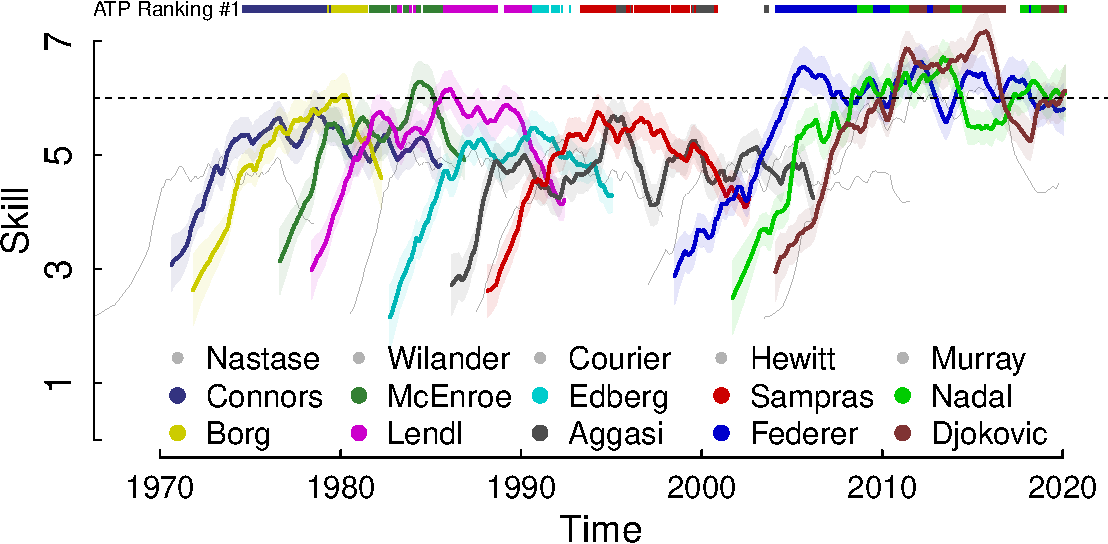
\includegraphics[width=\linewidth]{../static/atp.pdf}
\end{textblock}

\end{frame}


\begin{frame}[plain]
\begin{textblock}{160}(0,4)
\centering \Large Poster 2 \\  
\large 
Ventaja evolutva de la cooperación y la especialización.
\end{textblock}


\begin{textblock}{80}(0,18) \centering
\includegraphics[width=\linewidth]{../figures/pdf/ergodicity_individual_trayectories_y.pdf}
\end{textblock}

\begin{textblock}{80}(80,18) \centering
\includegraphics[width=\linewidth]{../figures/pdf/ergodicity_desertion.pdf}
\end{textblock}

\end{frame}



\end{document}
